\documentclass[a4paper]{article}
\usepackage[letterpaper, margin=1in]{geometry} % page format
\usepackage{listings,graphicx,amsmath, amssymb, amsfonts, amsthm, tikz, hyperref, fullpage, setspace, enumerate, mathtools, arydshln}
\usepackage[english]{babel}

\title{Homework 5}
\author{Helen Ngo}
\date{\today}

\begin{document}
\lstset{language=Python,basicstyle=\ttfamily\footnotesize}

\maketitle

\begin {description}

\item[Problem 1] Experiment with k-means for color quantization.

\begin{enumerate}[(e) i.]
\item Explain what happens when you increase or decrease the value of $n\_colors$?
\item Explain in what other possible applications do you think this can be useful?
\item Why do you think the resulting picture was funny at the end?
\end{enumerate}

\smallskip
\textbf{Soultion:}
\begin{doublespace}
\begin{enumerate}[(e) i.]
\item As the value of $n\_colors$ increase, the number of distinct colors possible in the given image increases. And as the value of $n\_colors$ decrease, the number of distinct colors possible in the given image decreases. Thus $n\_colors$ limits the color palette of an image and how the colors of the objects in the image are represented.
\item Color quantization is commonly used in GIF and PNG images, especially on the World Wide Web. A possible application for k-means for color quantization is in image processing. By limiting the number of colors in an image, the shape of certain objects can be more easily identified, especially from an image generated with thermography. For instance, a person's body has various temperatures depending on the part, so the thermal image of a person in an environment may seem cluttered. Color quantization can reduce the number of colors and thus number of shapes in the image will also be reduced, enabling the identification of the object of interest, probably the human.
\item The resulting picture, shown on the next page, was funny at the end because the reduced color palette limited the contours of the face that could be identified. The modified image looks flat and the features are hard to identified and reflection of light on the face are exaggerated.
\begin{center}
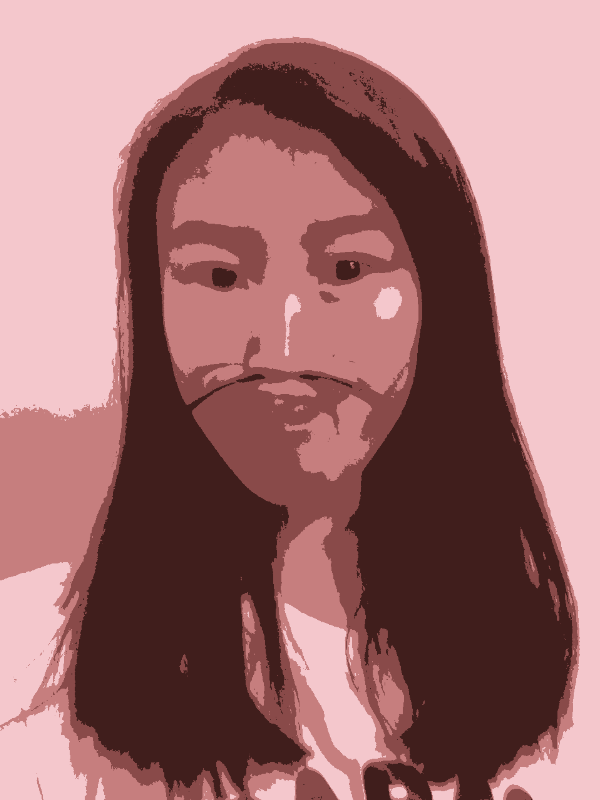
\includegraphics[scale=0.65]{funnyme.png}
\end{center}
\end{enumerate}
\end{doublespace}

\item[Problem 2] Neural networks: The MLP \\Explain your results. What do you think is happening? What is your interpretation of the number of neurons with respect to the performance of the network?

\smallskip
\textbf{Soultion:}
\begin{doublespace}
A the lowest number of neurons and lowest learning parameter is used. Iterations of MLP runs with those parameters. The learning parameter is increased and MLP runs. This is repeated for a the number of neurons until the error tolerance or max iterations is met. Then using cross-validation, an increased number of neurons and the lowest parameter is used. Repeated as before. 

As the number of neurons increase, so does the performance of the network in terms of accuracy. As the number samples increase, the number of neurons necessary for the desired performance is also increased.
\end{doublespace}
\end {description}
\end{document}
